\section{Tutorial -- Parameter Estimation}

\textbf{Note:} The NLopt solvers are used for the tutorial, but are an optional to the installation. See the install instructions for more information about installing NLopt.

This tutorial provides a very simple example of using the sampling with optimization. Sampling can be used to do optimization under uncertainty where there are several scenarios with differing values of uncertain parameters. Sampling can also be used to do parameter estimation, where estimated values must be compared against several data points. This tutorial will focus on parameter estimation.  

At any point in this tutorial, the FOQUS session can be saved and the tutorial can be started again from that point.

The model is given by Equation \ref{eq.pe.tut}.  The unknown parameters are $a$, $b$, and $c$. The x and y data are given in Table \ref{table.pe.data}.

\begin{equation}\label{eq.pe.tut}
y = ax^2 + bx + c
\end{equation}

\begin{table}[H]
	\begin{center}
		\caption{x-y Data}\label{table.pe.data}
		\begin{tabularx}{2.1in}{r r r r r r}
			\hline
			Sample  & 1 & 2 & 3 & 4 & 5 \\
			\hline
			x & 0 & 1 & 2 & 3  & 4 	 \\
			y & 1 & 0 & 3 & 10 & 21  \\
			\hline
		\end{tabularx}
	\end{center}
\end{table}

The first step is to create a flowsheet with one node.  The node will have the input variables: a, b, c, x, and ydata; and output variable y.
\begin{enumerate}
	\item Open FOQUS.
	\item In the \textbf{\underline{Session Name}} field, enter ``PE\_tutorial'' (see Figure \ref{fig.pe.tut1}).
	\item Click the \bu{Flowsheet} button in the top toolbar.
\end{enumerate}

\begin{figure}[H]
	\begin{center}
		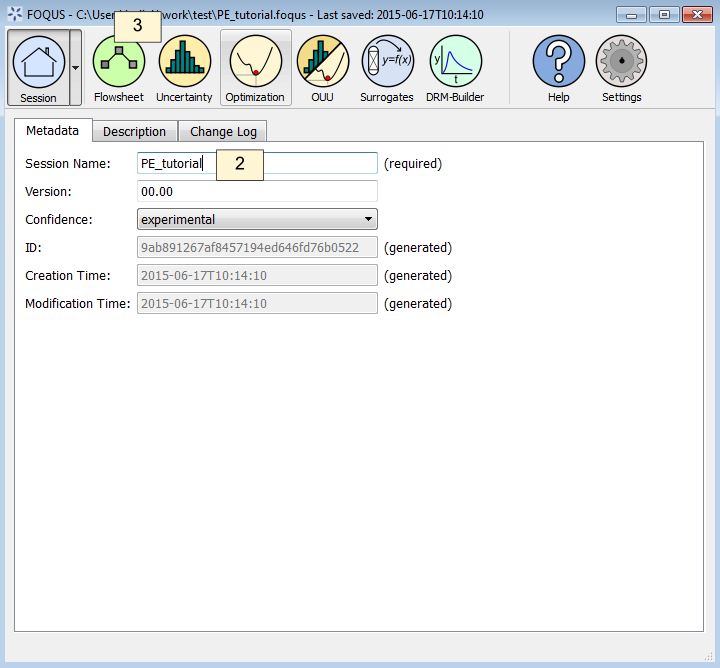
\includegraphics[scale=0.55]{Chapt_optimization/figs/par_est_tut1}
		\caption{Session Setup}
		\label{fig.pe.tut1}
	\end{center}
\end{figure}

\begin{enumerate}
	\setcounter{enumi}{3}
	\item Add a node to the flowsheet named ``model.''
	\begin{enumerate}
		\item Click \bu{Add Node} in the left toolbar (see Figure \ref{fig.pe.tut2}).
		\item Click anywhere on the gridded flowsheet area.
		\item Select ``model'' in the \textbf{\underline{Name}} drop-down list and then click \bu{OK}.
	\end{enumerate}
	\item Click the \bu{Selection Mode} icon in the left toolbar (see Figure \ref{fig.pe.tut2}).
	\item Click the \bu{Node Editor} icon in the left toolbar (see Figure \ref{fig.pe.tut2}).
	\item In the Node Edit input table, add the variables a, b, c, x, and ydata. The ydata variable will be used as an input for the known y sample point data, later in the tutorial.
	\begin{enumerate}
		\item Click the \bu{Add Input} icon  (see Figure \ref{fig.pe.tut2}).
		\item Enter ``a'' for the variable name in the \textbf{\underline{Name}} column.
		\item Enter -10 and 10 for the min and max in the \textbf{\underline{Min}} and \textbf{\underline{Max}} columns for a, b, c, and x.
		\item Repeat for all of the inputs.
		\item Enter 1 for the value of a, b, and c in the \textbf{\underline{Value}} column.
		\item Enter 2 for the value of x in the \textbf{\underline{Value}} column.
		\item The \textbf{\underline{Value}}, \textbf{\underline{Min}}, and \textbf{\underline{Max}} for ydata do not matter.
	\end{enumerate}
\end{enumerate}



\begin{figure}[H]
	\begin{center}
		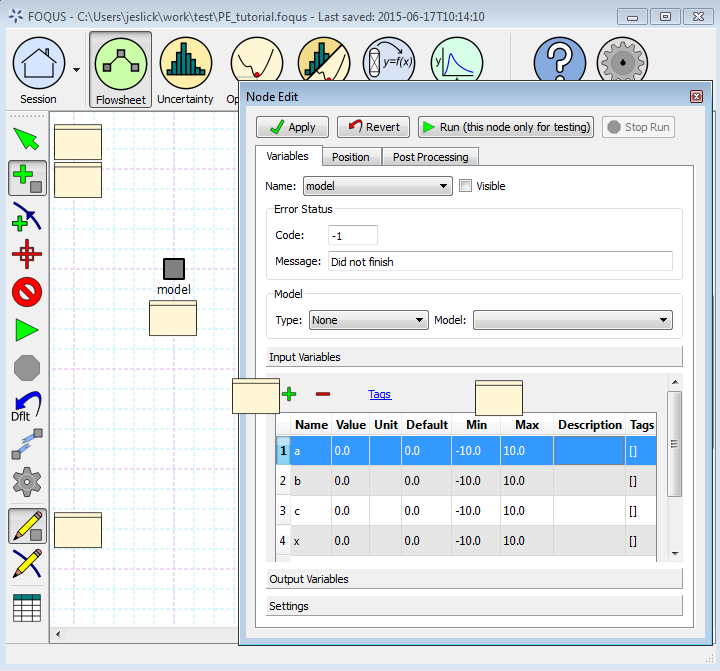
\includegraphics[scale=0.55]{Chapt_optimization/figs/par_est_tut2}
		\caption{Adding Node and Inputs}
		\label{fig.pe.tut2}
	\end{center}
\end{figure}

\begin{enumerate}
	\setcounter{enumi}{7}
	\item Click \bu{Output Variables} (see Figure \ref{fig.pe.tut3}).
	\item Add the output variable y.
	\begin{enumerate}
		\item Click the \bu{Add Output} icon (see Figure \ref{fig.pe.tut3}).
		\item Enter ``y'' for the variable name in the \textbf{\underline{Name}} column.
	\end{enumerate}
\end{enumerate}

\begin{figure}[H]
	\begin{center}
		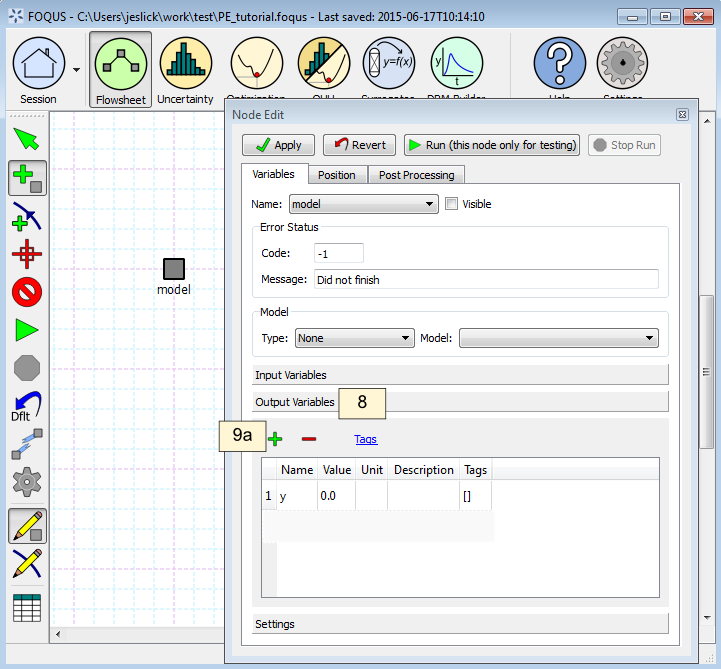
\includegraphics[scale=0.55]{Chapt_optimization/figs/par_est_tut3}
		\caption{Adding Outputs}
		\label{fig.pe.tut3}
	\end{center}
\end{figure}

\begin{enumerate}
	\setcounter{enumi}{9}
	\item Add the model equation to the node.
	\begin{enumerate}
		\item Click the \bu{Node Script} tab.
		\item Enter the following code in the calculations box:
		\begin{Verbatim}
f['y'] = x['a']*x['x']**2\
 + x['b']*x['x'] + x['c']
		\end{Verbatim}
	\end{enumerate}
\end{enumerate}

\begin{figure}[H]
	\begin{center}
		\includegraphics[scale=0.55]{Chapt_optimization/figs/par_est_tut4}
		\caption{Adding Node Calculation}
		\label{fig.pe.tut4}
	\end{center}
\end{figure}

\begin{enumerate}
	\setcounter{enumi}{10}
	\item Return to the Output Variables table in the Node Editor, by clicking on the \bu{Variables} tab, and selecting \bu{Output Variables}.
	\item Click \bu{Run} in the left toolbar in the FOQUS Home window, to test a single flowsheet evaluation and ensure there are no errors.
	\item When the run is complete, there should be no error and the value of y should be 7 in the Output Variables table.
\end{enumerate}

The next step is to setup the optimization. The objective function is to minimize the sum of the squared errors between the estimated value of y and the observed value of y. There are five data points in Table \ref{table.pe.data}, so there are five flowsheet evaluations that need to go into the calculation of the objective.

\begin{enumerate}
	\setcounter{enumi}{13}
	\item Click the \textbf{\underline{Optimization}} button in the top toolbar of the Home window (see Figure \ref{fig.pe.tut5}).
	\item Select ``Decision'' in the \textbf{\underline{Type}} column drop-down lists for ``model.a,'' ``model.b,'' and \\``model.c.'' The \textbf{\underline{Scale}} column will automatically be set to linear.
	\item Select ``Sample'' in the \textbf{\underline{Type}} column drop-down lists for ``model.x'' and ``model.ydata.''
\end{enumerate}

\begin{figure}[H]
	\begin{center}
		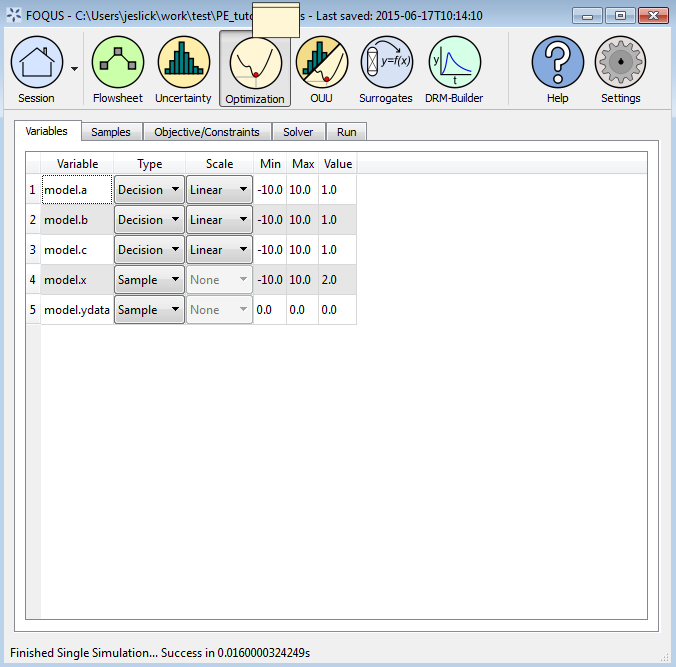
\includegraphics[scale=0.55]{Chapt_optimization/figs/par_est_tut5}
		\caption{Optimization Variables}
		\label{fig.pe.tut5}
	\end{center}
\end{figure}

The decision variables in the optimization problem will be changed by the optimization solver to try to minimize the objective, and the sample variables are used to construct the samples that will go into the objective function calculation.
\begin{enumerate}
	\setcounter{enumi}{16}
	\item Select the \bu{Samples} tab (see Figure \ref{fig.pe.tut6}).
	\item Click \bu{Add Sample} five times to add five samples.
	\item Enter the data from Table \ref{table.pe.data} in the Samples table.
	\item For larger sample sets, \bu{Generate Samples} has an option to load from a CSV file.
\end{enumerate}

\begin{figure}[H]
	\begin{center}
		\includegraphics[scale=0.55]{Chapt_optimization/figs/par_est_tut6}
		\caption{Optimization Samples}
		\label{fig.pe.tut6}
	\end{center}
\end{figure}

The objective function is the sum of the square difference between y and ydata for each sample in Table \ref{table.pe.data}. The optimization solver changes the a, b, and c to minimize the objective.

\begin{enumerate}
	\setcounter{enumi}{20}
	\item Click the \bu{Objective/Constraints} tab.
	\item Click the \bu{Add Objective} icon on the right side of the Objective Function table  (see Figure \ref{fig.pe.tut7}).
	\item In the \textbf{\underline{Expression}} column, enter the following (without the line break):
	\begin{small}
	\begin{verbatim}
sum([(f[i]['model']['y'][0] - x[i]['model']['ydata'][0])**2
 for i in range(len(x))])
	\end{verbatim}
	\end{small}
	The above expression uses Python list comprehension to calculate the sum of squared errors. The keys for x and f are: sample index, node name, variable name, time step.
	\item Enter 1 for the \textbf{\underline{Penalty Scale}}.
	\item Enter 100 for the \textbf{\underline{Value for Failure}}.
	\item No constraints are required.
\end{enumerate}

\begin{figure}[H]
	\begin{center}
		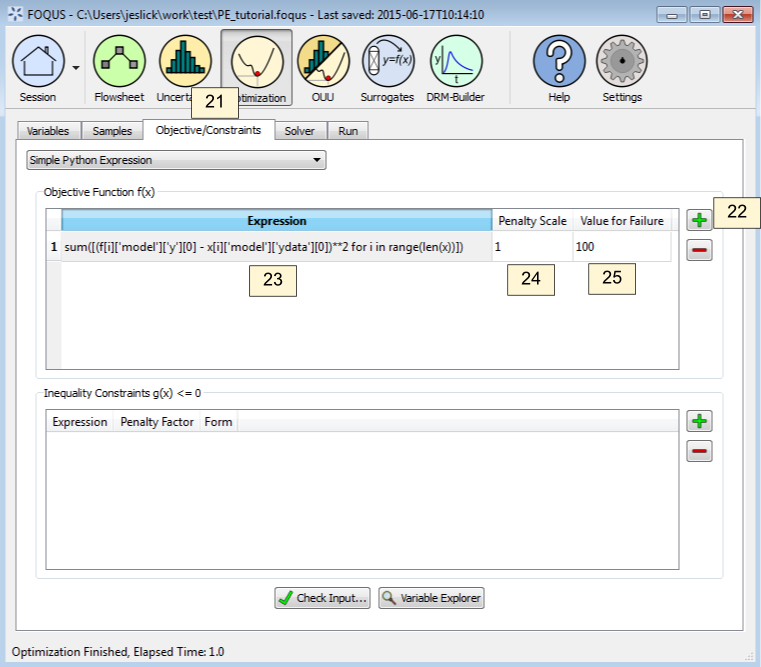
\includegraphics[scale=0.55]{Chapt_optimization/figs/par_est_tut7}
		\caption{Objective Function}
		\label{fig.pe.tut7}
	\end{center}
\end{figure}

Once the objective is set up, a solver needs to be selected and configured. Almost any solver in FOQUS should work well for this problem with the default values.

\begin{enumerate}
	\setcounter{enumi}{26}
	\item Click the \bu{Solver} tab (see Figure \ref{fig.pe.tut8}).
	\item Select ``NLopt'' from the \bu{Select Solver} drop-down list. NLopt is a collection of solvers that share a standard interface \citep{Johnson_2015}.
	\item Select ``BOBYQA'' under the Solver Options table in the \textbf{\underline{Settings}} column drop-down list.
\end{enumerate}

\begin{figure}[H]
	\begin{center}
		\includegraphics[scale=0.55]{Chapt_optimization/figs/par_est_tut8}
		\caption{Optimization Samples}
		\label{fig.pe.tut8}
	\end{center}
\end{figure}

\begin{enumerate}
	\setcounter{enumi}{29}
	\item Click the \bu{Run} tab (see Figure \ref{fig.pe.tut9}).
	\item Click the \bu{Start} button.
	\item The Optimization Solver Messages window displays the solver progress. As the solver runs, the best results found is placed into the flowsheet.
	\item The \textbf{\underline{Best Solution Parallel Coordinate Plot}} shows the scaled decision variable values for the best solution found so far.
	\item The \textbf{\underline{Objective Function Plot}} shows the value of the objective function as the optimization progresses.
\end{enumerate}

\begin{figure}[H]
	\begin{center}
		\includegraphics[scale=0.55]{Chapt_optimization/figs/par_est_tut9}
		\caption{Running Optimization}
		\label{fig.pe.tut9}
	\end{center}
\end{figure}

The best result at the end of the optimization is stored in the flowsheet. All flowsheet evaluations run during the optimization are stored in the flowsheet results table.

\begin{enumerate}
	\setcounter{enumi}{34}
	\item Once the optimization has completed, click \bu{Flowsheet} in the top toolbar.
	\item Open the \textbf{\underline{Node Editor}} and look at the \textbf{\underline{Input Variables}} table. The approximate result should be a = 2, b = -3, and c = 1  (see Figure \ref{fig.pe.tut10}).
\end{enumerate}
	
\begin{figure}[H]
	\begin{center}
		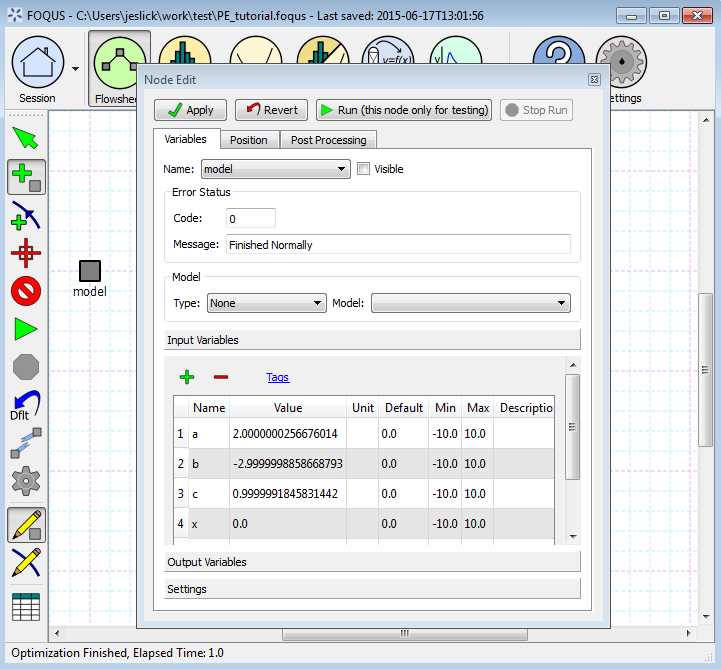
\includegraphics[scale=0.55]{Chapt_optimization/figs/par_est_tut10}
		\caption{Flowsheet, Input Variables Results}
		\label{fig.pe.tut10}
	\end{center}
\end{figure}
